%  BE Mini Project Report - CSDF (LP-IV)
%  Browser History Forensic Analysis Tool
%  Based on BE_PROJECT_REPORT_FORMAT_TERM_II_LATEX_FILE.tex (SPPU format)

\documentclass[oneside,a4paper,12pt]{report}

\usepackage{graphicx}
\usepackage{fancyhdr}
\usepackage{titlesec}
\usepackage{listings}
\usepackage{xcolor}
\usepackage{amsmath}
\usepackage[a4paper,margin=1in]{geometry}

\fancypagestyle{plain}{%
  \fancyhf{}
  \fancyfoot[C]{NBN SSOE, Department of Computer Engineering 2026-27}
  \fancyfoot[R]{\thepage}
}
\pagestyle{fancy}
\fancyhead{}
\renewcommand{\headrulewidth}{0pt}
\footskip = 0.625in
\cfoot{}
\rfoot{}

\usepackage[hidelinks]{hyperref}
\usepackage{tikz}
\usetikzlibrary{arrows,shapes,snakes,automata,backgrounds,petri,positioning,calc,fit}

\usepackage{tabularx}
\usepackage[nottoc,notlot,notlof,numbib]{tocbibind}
\usepackage[titletoc]{appendix}
\renewcommand{\appendixname}{Annexure}
\usepackage{titletoc}
\renewcommand{\bibname}{References}
\setcounter{secnumdepth}{5}
\usepackage{float}
\usepackage{subcaption}
\usepackage{multirow}
\usepackage[ruled,vlined]{algorithm2e}

% report class has no \frontmatter / \mainmatter
\newcommand{\frontmatter}{\clearpage\pagenumbering{roman}}
\newcommand{\mainmatter}{\clearpage\pagenumbering{arabic}\setcounter{page}{1}}

\lstset{basicstyle=\ttfamily\footnotesize, breaklines=true, frame=single,
  columns=fullflexible, keepspaces=true, showstringspaces=false,
  keywordstyle=\color{blue}, commentstyle=\color{gray}, stringstyle=\color{red!60!black}}

\newcommand{\ptitle}{Design and Development of a Browser History Forensic Analysis Tool}
\newcommand{\ptitleshort}{Browser History Forensic Analysis Tool}

\begin{document}

\setlength{\parindent}{0mm}
\begin{center}

\includegraphics[width=70pt]{sppulogo.jpg}\\
{\bfseries SAVITRIBAI PHULE PUNE UNIVERSITY \\}
 \vspace*{1\baselineskip}
{\bfseries A  MINI PROJECT REPORT ON \\}
 \vspace*{2\baselineskip}
{\bfseries \fontsize{16}{12} \selectfont \ptitle \\ \vspace*{2\baselineskip}}
{\fontsize{12}{12} \selectfont SUBMITTED TOWARDS THE
 \\PARTIAL FULFILLMENT OF THE REQUIREMENTS OF \\
 LABORATORY PRACTICE IV (CYBER SECURITY AND DIGITAL FORENSICS)\\
\vspace*{2\baselineskip}}
{\bfseries \fontsize{14}{12} \selectfont BACHELOR OF ENGINEERING (Computer
Engineering) \\
\vspace*{1\baselineskip}}
{\bfseries \fontsize{14}{12} \selectfont BY \\
\vspace*{1\baselineskip}}
Vishwajeet Tulse  \hspace{25 mm} Exam No: \underline{\hspace{25mm}}  \\
Student Name 2 \hspace{25 mm} Exam No: \underline{\hspace{25mm}}   \\
Student Name 3 \hspace{25 mm} Exam No: \underline{\hspace{25mm}}  \\
Student Name 4 \hspace{25 mm} Exam No: \underline{\hspace{25mm}}\\
\vspace*{2\baselineskip}
{\bfseries \fontsize{14}{12} \selectfont Under The Guidance of \\
\vspace*{1\baselineskip}}
Prof. Guide Name\\
\vspace*{1\baselineskip}

\includegraphics[width=100pt]{SinhgadLogo.jpg} \\
{\bfseries \fontsize{14}{12} \selectfont DEPARTMENT OF COMPUTER ENGINEERING \\
NBN SINHGAD SCHOOL OF ENGINEERING \\
10/1, AMBEGAON (BK), PUNE-411041 \\
2026-27
}
\end{center}

\newpage

\begin{figure}[ht]
\centering

\includegraphics[width=100pt]{SinhgadLogo.jpg}
\end{figure}

{\bfseries \fontsize{14}{12} \selectfont \centerline{NBN SINHGAD SCHOOL OF ENGINEERING}
\centerline{DEPARTMENT OF COMPUTER ENGINEERING}
\vspace*{2\baselineskip}}

{\bfseries \fontsize{16}{12} \selectfont \centerline{CERTIFICATE}
\vspace*{2\baselineskip}}

\centerline{This is to certify that the Mini Project Entitled}
\vspace*{.5\baselineskip}

{\bfseries \fontsize{14}{12} \selectfont \centerline{\ptitleshort}
\vspace*{0.5\baselineskip}}

\centerline{Submitted by}
\vspace*{0.5\baselineskip}
\centerline{Vishwajeet Tulse  \hspace{25 mm} Exam No: \underline{\hspace{25mm}} }
\centerline{Student Name 2 \hspace{25 mm} Exam No: \underline{\hspace{25mm}}  }
\centerline{Student Name 3 \hspace{25 mm} Exam No: \underline{\hspace{25mm}} }
\centerline{Student Name 4 \hspace{25 mm} Exam No: \underline{\hspace{25mm}} }
\vspace*{0.5\baselineskip}

is a bonafide work carried out by Students under the supervision of Prof. Guide Name and it
is submitted towards the partial fulfillment of the requirement of Bachelor of Engineering (Computer Engineering) for the course Laboratory Practice IV.\\

\bgroup
\def\arraystretch{0.7}
\vspace*{0.5\baselineskip}
\begin{tabular}{c c }
Prof. Guide Name &  \hspace{50 mm} Dr. S. P. Bendale \\
Internal Guide   &  \hspace{50 mm} H.O.D \\
Dept. of Computer Engg.  &	\hspace{50 mm}Dept. of Computer Engg.  \\
\end{tabular}
\egroup
\vspace*{0.5\baselineskip}
\begin{center}
{
Dr. S. P. Patil \\
Principal\\
NBN Sinhgad School of Engineering
}
\end{center}
\vspace*{1\baselineskip}
Signature of Internal Examiner \hspace{30 mm} Signature of External Examiner
\newpage

\begin{center}
\textbf{PROJECT APPROVAL SHEET}
\end{center}
\begin{center}
 \ptitle
 \end{center}
\begin{center}
Is successfully completed by
\end{center}
\centerline{Vishwajeet Tulse  \hspace{25 mm} Exam No: \underline{\hspace{25mm}} }
\centerline{Student Name 2 \hspace{25 mm} Exam No: \underline{\hspace{25mm}}  }
\centerline{Student Name 3 \hspace{25 mm} Exam No: \underline{\hspace{25mm}} }
\centerline{Student Name 4 \hspace{25 mm} Exam No: \underline{\hspace{25mm}} }
\begin{center}
 at
 \end{center}
 \begin{center}
 DEPARTMENT OF COMPUTER ENGINEERING
 \end{center}
 \begin{center}
 NBN SINHGAD SCHOOL OF ENGINEERING, PUNE
 \end{center}
 \begin{center}
 SAVITRIBAI PHULE PUNE UNIVERSITY, PUNE
 \end{center}
 \begin{center}
 ACADEMIC YEAR 2026-2027
 \end{center}
 \vspace*{1\baselineskip}
 \begin{tabular}{c c }
Prof. Guide Name &  \hspace{50 mm} Dr. S. P. Bendale \\
Internal Guide   &  \hspace{50 mm} H.O.D \\
Dept. of Computer Engg.  &	\hspace{50 mm}Dept. of Computer Engg.  \\
\end{tabular}
\newpage

\setcounter{page}{0}
\frontmatter
\cfoot{NBN SSOE, Department of Computer Engineering 2026-27}
\rfoot{\thepage}
\pagenumbering{Roman}

{  \newpage {\bfseries \fontsize{14}{12} \selectfont \centerline{Abstract}
\vspace*{2\baselineskip}} \setlength{\parindent}{11mm} }
{ \setlength{\parindent}{0mm} }
Web browsers record every page a user opens, every search they make and every file they download. In a digital-forensic investigation this browsing history is one of the richest sources of evidence about a suspect's activity, intent and timeline. Modern Chromium-based browsers (Google Chrome, Microsoft Edge, Brave) store this history in a single SQLite database called \texttt{History}, but the data is not directly readable: the file is locked while the browser runs, timestamps are stored as microseconds since 1 January 1601, and the information is spread across several related tables.

This mini project presents the design and development of a \textbf{Browser History Forensic Analysis Tool} that automates the standard forensic workflow of \emph{acquire, preserve, analyse and report}. The tool copies the History database to a working location, computes and verifies a SHA-256 hash of the evidence so that its integrity can be demonstrated, parses the \texttt{urls}, \texttt{visits} and \texttt{downloads} tables, converts WebKit timestamps into human-readable local time, and produces a chronological timeline of browsing activity. It further summarises the most visited domains, daily activity, downloaded files and keyword hits, and exports the results as CSV files and a self-contained HTML report that can be attached to an investigation file.

The tool is written in about 280 lines of Python using only the standard library (\texttt{sqlite3}, \texttt{hashlib}, \texttt{csv}, \texttt{argparse}), so it runs on Windows, Linux and macOS without installing any third-party package. A sample database generator and a pytest suite of seven tests are included, and the tool was verified on a synthetic database and on the live Microsoft Edge history of a Windows 11 machine. The outcome is a small, transparent and easily explainable forensic utility that demonstrates the core principles of evidence handling, artifact parsing and timeline analysis taught in the Cyber Security and Digital Forensics course.

{  \newpage {\bfseries \fontsize{14}{12} \selectfont \centerline{Acknowledgments}
\vspace*{2\baselineskip}} \setlength{\parindent}{11mm} }
{ \setlength{\parindent}{0mm} }
\textit{It gives us great pleasure in presenting the mini project report
on {\bfseries \fontsize{12}{12} \selectfont `\ptitleshort'}.}
\vspace*{1.5\baselineskip}

 \textit{We would like to take this opportunity to thank our internal guide
 \textbf{Prof. Guide Name} for giving us all the help and guidance we needed. We are
 really grateful to them for their kind support. Their valuable suggestions were very helpful.} \vspace*{1.5\baselineskip}

 \textit{We are also grateful to \textbf{Dr. S. P. Bendale}, Head of Computer
 Engineering Department, NBN Sinhgad School of Engineering, for his indispensable
 support and suggestions.}
\vspace*{1.5\baselineskip}

\textit{In the end our special thanks to the \textbf{laboratory staff of the Department of Computer Engineering} for
providing various resources such as the laboratory with all needed software platforms and
continuous Internet connection for our project.}
\vspace*{3\baselineskip} \\
\begin{tabular}{p{8.2cm}c}
&Vishwajeet Tulse\\
&Student Name 2\\
&Student Name 3\\
&Student Name 4\\
&(B.E. Computer Engg.)
\end{tabular}

\tableofcontents
\listoffigures
\listoftables

\mainmatter

\titleformat{\chapter}[display]
{\fontsize{16}{15}\filcenter}
{\vspace*{\fill}
 \bfseries\LARGE\MakeUppercase{\chaptertitlename}~\thechapter}
{1pc}
{\bfseries\LARGE\MakeUppercase}
[\thispagestyle{empty}\vspace*{\fill}\newpage]

\setlength{\parindent}{11mm}

% =====================================================================
\chapter{Synopsis}

\section{Project Title}
\ptitle

\section{Project Option}
Internal project (mini project for Laboratory Practice IV, Cyber Security and Digital Forensics).

\section{Internal Guide}
Prof. Guide Name

\section{Sponsorship and External Guide}
Not applicable. The project is not sponsored.

\section{Technical Keywords (As per ACM Keywords)}
\begin{enumerate}
  \item Security and privacy
  \begin{enumerate}
    \item Security services
    \begin{enumerate}
      \item Digital forensics
      \item Data integrity (cryptographic hashing)
    \end{enumerate}
  \end{enumerate}
  \item Information systems
  \begin{enumerate}
    \item Data management systems
    \begin{enumerate}
      \item Relational database query languages (SQLite / SQL)
    \end{enumerate}
  \end{enumerate}
  \item Software and its engineering
  \begin{enumerate}
    \item Software notations and tools
    \begin{enumerate}
      \item Command line tools, scripting languages (Python)
    \end{enumerate}
  \end{enumerate}
\end{enumerate}

\section{Problem Statement}
\label{sec:problem}
Design and develop a digital-forensic tool that acquires the browsing-history database of a Chromium-based web browser (Chrome, Edge, Brave), preserves its integrity using cryptographic hashing, parses the visited URLs, page titles, timestamps and downloads, and generates a chronological timeline with summary statistics, keyword search and an exportable report for use in a forensic investigation.

\section{Abstract}
\begin{itemize}
  \item Browser history is a key artifact in cyber-crime investigations because it reveals what a user searched for, which sites were visited, when, and what was downloaded.
  \item Chromium browsers keep this data in a locked SQLite file with non-standard timestamps, so it cannot be examined directly or safely.
  \item The proposed tool copies the evidence, verifies it with SHA-256, parses it with the Python \texttt{sqlite3} module, converts WebKit time to local time and builds a timeline.
  \item It reports the top visited domains, daily activity, downloads and keyword hits, and exports CSV and HTML reports.
  \item The implementation is a single Python file with no third-party dependencies, accompanied by a sample-database generator and automated tests.
\end{itemize}

\section{Goals and Objectives}
\begin{itemize}
  \item To understand how Chromium-based browsers store browsing history and downloads.
  \item To acquire the History database without altering the original evidence and to prove integrity using SHA-256.
  \item To convert WebKit/Chrome timestamps into readable local date-time values.
  \item To reconstruct a chronological timeline of user activity.
  \item To provide analysis features useful to an investigator: top domains, daily activity, keyword search and download listing.
  \item To generate CSV and HTML reports that can be attached to a case file.
  \item To keep the tool small, portable and easy to explain.
\end{itemize}

\section{Relevant mathematics associated with the Project}
\label{sec:math}
System Description:
\begin{itemize}
\item \textbf{Input:} $H$ = the browser History SQLite file; $k$ = optional keyword; $n$ = number of top domains.
\item \textbf{Output:} evidence copy $H'$ with hash $h = \mathrm{SHA256}(H)$; ordered timeline $T = \langle t_1, t_2, \dots, t_m \rangle$; domain frequency table $D$; keyword hit set $K$; downloads list $L$; files \texttt{timeline.csv}, \texttt{downloads.csv}, \texttt{report.html}.
\item \textbf{Data structures:} list of visit dictionaries (time, url, title, domain, visit\_count, typed\_count); \texttt{Counter} (hash map) for domain and daily frequencies; SQL join of relations \texttt{visits} $\bowtie$ \texttt{urls}.
\item \textbf{Functions:}
  \begin{itemize}
    \item $f_{acq}: H \rightarrow (H', h)$ with the success condition $\mathrm{SHA256}(H) = \mathrm{SHA256}(H')$.
    \item $f_{time}: \mu \rightarrow t$, where $t = \mu / 10^{6} - 11644473600$ seconds since the Unix epoch ($\mu$ = microseconds since 1601-01-01).
    \item $f_{parse}: H' \rightarrow T$, $T$ sorted by visit time.
    \item $f_{top}: (T, n) \rightarrow D$, the $n$ most frequent domains.
    \item $f_{key}: (T, k) \rightarrow K = \{ v \in T \mid k \subseteq \mathrm{lower}(v.url) \lor k \subseteq \mathrm{lower}(v.title) \}$.
  \end{itemize}
\item \textbf{Mathematical formulation:} the timeline is a totally ordered set under visit time; domain ranking is a frequency count $D(d) = |\{ v \in T : \mathrm{domain}(v) = d \}|$. Complexity is $O(m \log m)$ for sorting (done by SQLite) and $O(m)$ for every analysis pass.
\item \textbf{Success Conditions:} History file is found and readable; hash of copy equals hash of source; timeline and reports are produced.
\item \textbf{Failure Conditions:} file not found; file is not a valid SQLite database or lacks the expected tables; hash mismatch after copy (tool aborts to protect integrity).
\end{itemize}

\section{Names of Conferences / Journals where papers can be published}
\begin{itemize}
\item IEEE International Conference on Computing, Communication and Networking Technologies (ICCCNT)
\item Digital Investigation / Forensic Science International: Digital Investigation (Elsevier)
\item International Conference on Digital Forensics and Cyber Crime (ICDF2C)
\item SPPU-sponsored and IIT-hosted student technical conferences / workshops
\end{itemize}

\section{Review of Conference/Journal Papers supporting Project idea}
\label{sec:survey}
A brief review of the literature consulted is given below; the detailed survey is in Chapter 3.
\begin{enumerate}
  \item Oh, Lee and Lee \cite{oh2011} describe browser log analysis as a central step in digital investigations and propose a timeline-based methodology, which this project follows.
  \item Ohana and Shashidhar \cite{ohana2013} show that private-browsing and portable browsers still leave recoverable artifacts, motivating careful acquisition.
  \item Rathod \cite{rathod2017} documents the Chrome artifacts (History, Cookies, Login Data) and their SQLite structure.
  \item Casey \cite{casey2011} and Carrier \cite{carrier2005} give the general principles of evidence integrity and file-system forensics used for the acquisition step.
  \item The Chromium project documentation \cite{chromiumhist} and the SQLite documentation \cite{sqlite} define the schema and the file format parsed by the tool.
  \item Kessler \cite{kessler2016} explains cryptographic hashing (MD5/SHA) as the standard integrity mechanism in forensics.
  \item NIST SP 800-86 \cite{nist80086} provides the four-phase model (collection, examination, analysis, reporting) adopted as the tool's architecture.
  \item Pressman \cite{bookPressman} is used for the project-planning and risk-analysis framework.
\end{enumerate}

\section{Plan of Project Execution}
The project was executed in five short phases over four weeks: (1) study of Chromium History schema and forensic principles, (2) design of the acquire-parse-analyse-report pipeline, (3) implementation in Python, (4) testing with a synthetic database and a live Edge profile, (5) report preparation. See Annexure C for the planner.

% =====================================================================
\chapter{Technical Keywords}
\section{Area of Project}
Cyber Security and Digital Forensics: browser artifact analysis, evidence acquisition and integrity verification.

\section{Technical Keywords}
\begin{enumerate}
  \item Security and privacy
  \begin{enumerate}
    \item Digital forensics
    \item Hash functions and message authentication codes
  \end{enumerate}
  \item Information systems
  \begin{enumerate}
    \item Structured Query Language, relational databases (SQLite)
  \end{enumerate}
  \item Applied computing
  \begin{enumerate}
    \item Computer forensics, evidence collection, timeline analysis
  \end{enumerate}
  \item Software and its engineering
  \begin{enumerate}
    \item Scripting languages (Python), command-line tools, software testing (pytest)
  \end{enumerate}
\end{enumerate}

% =====================================================================
\chapter{Introduction}
\section{Project Idea}
\begin{itemize}
\item Every Chromium-based browser keeps a per-profile SQLite file named \texttt{History} containing the tables \texttt{urls} (one row per unique URL with title and visit counts), \texttt{visits} (one row per visit with a timestamp) and \texttt{downloads}.
\item The idea is to build a small forensic tool that reads this file in a forensically sound way and turns the raw rows into information an investigator can use: a timeline, frequency statistics, keyword hits and a printable report.
\item The tool is deliberately kept simple: one Python file, standard library only, command-line interface, so that each step can be explained and verified.
\end{itemize}

\section{Motivation of the Project}
\begin{itemize}
\item Commercial forensic suites (EnCase, FTK, Magnet AXIOM) are expensive and act as black boxes; students rarely get to see how an artifact is actually parsed.
\item The LP-IV syllabus asks for a tool for digital forensics of a user artifact; browser history is universal, easily available and highly relevant to real cases (phishing, fraud, data exfiltration, insider threats).
\item Building the parser by hand teaches three essential forensic concepts at once: evidence integrity (hashing), artifact structure (SQLite schema) and timeline reconstruction (timestamp conversion and ordering).
\end{itemize}

\section{Literature Survey}
\begin{itemize}
\item \textbf{Oh, Lee and Lee (2011)} \cite{oh2011} proposed an advanced methodology for web-browser log analysis that integrates history, cache and cookies into a single timeline and highlights searched keywords. Our tool implements the history-and-download part of this methodology.
\item \textbf{Ohana and Shashidhar (2013)} \cite{ohana2013} examined private and portable browsing sessions and found that significant artifacts remain on disk, confirming that the History database is a reliable evidence source.
\item \textbf{Rathod (2017)} \cite{rathod2017} analysed Google Chrome's forensic artifacts on Windows, listing the History, Cookies, Login Data and Top Sites SQLite files and their key columns; the \texttt{urls}/\texttt{visits} join used here follows that description.
\item \textbf{Casey (2011)} \cite{casey2011} sets out the principles of digital evidence handling, including working on a verified copy rather than the original.
\item \textbf{Carrier (2005)} \cite{carrier2005} explains file-system level analysis and the role of hashing in proving that an image has not changed.
\item \textbf{NIST SP 800-86 (2006)} \cite{nist80086} defines the collection, examination, analysis and reporting phases; the tool's four steps map directly to these phases.
\item \textbf{Kessler (2016)} \cite{kessler2016} gives an overview of cryptographic hash functions and why SHA-256 is preferred over MD5 for evidence verification today.
\item \textbf{Chromium design documentation} \cite{chromiumhist} documents the WebKit time format: a 64-bit count of microseconds since 1 January 1601 UTC, which must be shifted by 11\,644\,473\,600 seconds to obtain Unix time.
\item \textbf{SQLite documentation} \cite{sqlite} describes the single-file database format and the read-only URI mode used to open the evidence copy without modification.
\item \textbf{Python documentation} \cite{pydocs} for the \texttt{sqlite3}, \texttt{hashlib} and \texttt{datetime} modules used in the implementation.
\end{itemize}

% =====================================================================
\chapter{Problem Definition and scope}
\section{Problem Statement}
Investigators need to know what a user did in a web browser and when. The required information exists in the browser's History database, but it is locked by the running browser, uses a non-standard timestamp format and is spread over several tables. Reading it manually is slow and error-prone, and opening the original file risks modifying the evidence. The problem is therefore to build a tool that \emph{safely acquires} the History file, \emph{verifies} its integrity, \emph{parses} it into a readable timeline and \emph{reports} the findings.

\subsection{Goals and objectives}
\begin{itemize}
  \item Input: path of a History file, or the name of a browser (\texttt{chrome}, \texttt{edge}, \texttt{brave}) from which the default path is derived; optional keyword and top-$n$ value.
  \item Output: an evidence copy with its SHA-256 digest, \texttt{timeline.csv}, \texttt{downloads.csv} and \texttt{report.html}, plus a console summary.
  \item Objective: correctness of timestamps, completeness of the timeline, preservation of the original, and a clear report.
\end{itemize}

\subsection{Statement of scope}
\begin{itemize}
  \item The tool handles Chromium-family browsers (Chrome, Edge, Brave) on Windows, Linux and macOS. The History file is typically a few hundred kilobytes to a few hundred megabytes; the tool reads it in a single pass.
  \item Input validation: the path must exist and must be a SQLite database with \texttt{urls} and \texttt{visits} tables; the \texttt{downloads} table is optional.
  \item The tool \emph{does} produce timelines, domain statistics, daily activity, keyword hits and download lists.
  \item The tool \emph{does not} parse Firefox (\texttt{places.sqlite}), cookies, cache, saved passwords or deleted (free-page) records, and it does not modify the source file.
\end{itemize}

\section{Major Constraints}
\begin{itemize}
  \item The original History file must never be written to; the tool opens only the copy, in read-only mode.
  \item Only the Python standard library may be used, so the tool runs on an examiner workstation without Internet access.
  \item Browser History schema may change between versions; the tool uses only long-stable columns (\texttt{url}, \texttt{title}, \texttt{visit\_time}, \texttt{visit\_count}, \texttt{typed\_count}, \texttt{target\_path}, \texttt{tab\_url}, \texttt{start\_time}).
  \item Reading a live user profile requires that the examiner has file-system access to the profile folder.
\end{itemize}

\section{Methodologies of Problem solving and efficiency issues}
\begin{itemize}
  \item \textbf{Manual inspection with a SQLite GUI:} possible but slow, offers no hashing, no timestamp conversion and no reporting.
  \item \textbf{Commercial forensic suite:} complete but costly and opaque; unsuitable for a learning project.
  \item \textbf{Chosen approach, custom Python script:} a single SQL join retrieves all visits ordered by time ($O(m \log m)$ inside SQLite), and each analysis pass is linear in the number of visits. A 100\,000-visit database is processed in well under a second; the HTML report is generated with string concatenation, which is adequate for this size.
\end{itemize}

\section{Outcome}
\begin{itemize}
  \item A working command-line forensic tool (\texttt{bhft.py}) with hashing, parsing, analysis and reporting.
  \item A synthetic History generator for safe demonstrations and a pytest suite that verifies every function.
  \item A documented GitHub repository and this report.
\end{itemize}

\section{Applications}
\begin{itemize}
  \item Cyber-crime investigation: establishing which websites a suspect visited and when.
  \item Corporate incident response: checking whether a phishing link was opened or a malicious file downloaded.
  \item Insider-threat and data-leak investigations: identifying uploads to file-sharing or webmail sites.
  \item Parental or institutional policy audits, and teaching of digital forensics.
\end{itemize}

\section{Hardware Resources Required}
\begin{table}[!htbp]
\begin{center}
\def\arraystretch{1.5}
  \begin{tabular}{| c | c | c | p{5.5cm} |}
\hline
Sr. No. &	Parameter &	Minimum Requirement & Justification \\
\hline
1 &	CPU Speed &	 1 GHz  & Parsing is linear; any modern CPU suffices\\
\hline
2 &	RAM  &	2 GB &  The whole History table is held in memory; typical files are well under 100 MB\\
\hline
3 &	Disk  &	500 MB free &  Space for the evidence copy and reports\\
\hline
\end{tabular}
 \caption { Hardware Requirements }
 \label{tab:hreq}
\end{center}
\end{table}

\section{Software Resources Required}
Platform :
\begin{enumerate}
\item Operating System: Windows 10/11, Linux or macOS
\item IDE: Visual Studio Code (any text editor is sufficient)
\item Programming Language: Python 3.9 or newer (standard library only); pytest for the test suite
\item Browser for viewing the HTML report; Git and GitHub for version control
\end{enumerate}

% =====================================================================
\chapter{Project Plan}

\section{Project Estimates}
The project followed a simple waterfall model: requirements, design, implementation, testing and documentation.
\subsection{Reconciled Estimates}
\subsubsection{Cost Estimate}
All software used is free and open source (Python, pytest, Git, VS Code, MiKTeX). The only cost is student effort, estimated at 40 person-hours for a team of four, and use of existing laboratory computers.

\subsubsection{Time Estimates}
\begin{table}[!htbp]
\begin{center}
\def\arraystretch{1.3}
\begin{tabular}{| l | c |}
\hline
Phase & Duration \\ \hline
Study of History schema and forensic principles & 4 days \\ \hline
Design (pipeline, data structures, CLI) & 2 days \\ \hline
Implementation of \texttt{bhft.py} and sample generator & 5 days \\ \hline
Testing (pytest, live Edge profile) & 3 days \\ \hline
Report and repository documentation & 4 days \\ \hline
\textbf{Total} & \textbf{18 working days} \\ \hline
\end{tabular}
\caption{Time estimates}
\label{tab:time}
\end{center}
\end{table}

\subsection{Project Resources}
People: four students and one guide. Hardware: one laptop per student. Software: Python 3, pytest, Git/GitHub, VS Code, Microsoft Edge (for a live test profile), MiKTeX for the report.

\section{Risk Management w.r.t. NP Hard analysis}
The problem is not NP-hard: every step is a linear or $O(m \log m)$ pass over the visit rows. Risks are therefore practical rather than computational.
\subsection{Risk Identification}
Risks were identified by reviewing the scope and the environment in which the tool runs, using the questionnaire suggested in \cite{bookPressman}. The relevant answers: requirements are stable and fully understood; the team has the required Python skills; end-user expectations (a simple timeline tool) are realistic.

\subsection{Risk Analysis}
\begin{table}[!htbp]
\begin{center}
\def\arraystretch{1.5}
\begin{tabularx}{\textwidth}{| c | X | c | c | c | c |}
\hline
\multirow{2}{*}{ID} & \multirow{2}{*}{Risk Description}	& \multirow{2}{*}{Probability} & \multicolumn{3}{|c|}{Impact} \\ \cline{4-6}
	& & &	Schedule	& Quality	& Overall \\ \hline
1	& Browser History schema changes in a new version	& Low	& Low	& High	& Medium \\ \hline
2	& Locked History file cannot be copied while browser runs	& Medium	& Low	& Medium	& Medium \\ \hline
3	& Wrong timestamp conversion produces incorrect timeline	& Low	& Low	& Very high	& High \\ \hline
\end{tabularx}
\end{center}
\caption{Risk Table}
\label{tab:risk}
\end{table}

\begin{table}[!htbp]
\begin{center}
\def\arraystretch{1.5}
\begin{tabular}{| c | c | c |}
\hline
Probability & Value &	Description \\ \hline
High &	Probability of occurrence is &  $ > 75 \% $ \\ \hline
Medium &	Probability of occurrence is  & $26-75 \% $ \\ \hline
Low	& Probability of occurrence is & $ < 25 \% $ \\ \hline
\end{tabular}
\end{center}
\caption{Risk Probability definitions \cite{bookPressman}}
\label{tab:riskdef}
\end{table}

\begin{table}[!htbp]
\begin{center}
\def\arraystretch{1.5}
\begin{tabularx}{\textwidth}{| c | c | X |}
\hline
Impact & Value	& Description \\ \hline
Very high &	$> 10 \%$ & Schedule impact or Unacceptable quality \\ \hline
High &	$5-10 \%$ & Schedule impact or Some parts of the project have low quality \\ \hline
Medium	& $ < 5 \% $ & Schedule impact or Barely noticeable degradation in quality \\ \hline
\end{tabularx}
\end{center}
\caption{Risk Impact definitions \cite{bookPressman}}
\label{tab:riskImpactDef}
\end{table}

\subsection{Overview of Risk Mitigation, Monitoring, Management}
\begin{table}[!htbp]
\begin{center}
\def\arraystretch{1.5}
\begin{tabularx}{\textwidth}{| l | X |}
\hline
Risk ID	& 1 \\ \hline
Risk Description	& Browser History schema changes in a new version \\ \hline
Category	& Technology \\ \hline
Source	& Study of Chromium source and release notes \\ \hline
Probability	& Low \\ \hline
Impact	& High \\ \hline
Response	& Mitigate \\ \hline
Strategy	& Use only long-stable columns; wrap the optional \texttt{downloads} query in a try/except so the tool degrades gracefully \\ \hline
Risk Status	& Mitigated \\ \hline
\end{tabularx}
\end{center}
\end{table}

\begin{table}[!htbp]
\begin{center}
\def\arraystretch{1.5}
\begin{tabularx}{\textwidth}{| l | X |}
\hline
Risk ID	& 2 \\ \hline
Risk Description	& Locked History file cannot be read while the browser runs \\ \hline
Category	& Development Environment \\ \hline
Source	& Observed during testing on a live Edge profile \\ \hline
Probability	& Medium \\ \hline
Impact	& Medium \\ \hline
Response	& Mitigate \\ \hline
Strategy	& Copy the file with \texttt{shutil.copy2} (a byte copy is allowed even when SQLite holds a lock) and open only the copy in read-only mode \\ \hline
Risk Status	& Mitigated \\ \hline
\end{tabularx}
\end{center}
\end{table}

\begin{table}[!htbp]
\begin{center}
\def\arraystretch{1.5}
\begin{tabularx}{\textwidth}{| l | X |}
\hline
Risk ID	& 3 \\ \hline
Risk Description	& Wrong timestamp conversion \\ \hline
Category	& Requirements / Technology \\ \hline
Source	& Chromium documentation review \\ \hline
Probability	& Low \\ \hline
Impact	& Very High \\ \hline
Response	& Mitigate \\ \hline
Strategy	& Unit test that converts the known WebKit value of the Unix epoch and checks the result is 1970-01-01 \\ \hline
Risk Status	& Mitigated (test passes) \\ \hline
\end{tabularx}
\end{center}
\end{table}

\section{Project Schedule}
\subsection{Project task set}
Major Tasks in the Project stages are:
\begin{itemize}
  \item Task 1: Study Chromium History schema, WebKit time format and forensic acquisition principles.
  \item Task 2: Design the four-step pipeline and the command-line interface.
  \item Task 3: Implement acquisition, parsing, analysis and reporting functions.
  \item Task 4: Build the sample-database generator and the pytest suite; test on a live profile.
  \item Task 5: Prepare the GitHub repository and this report.
\end{itemize}

\subsection{Task network}
Task 1 $\rightarrow$ Task 2 $\rightarrow$ Task 3 $\rightarrow$ Task 4 $\rightarrow$ Task 5. Task 4 (sample generator) was started in parallel with Task 3 because the tests needed a database before the parser was complete.

\subsection{Timeline Chart}
\begin{figure}[H]
\centering
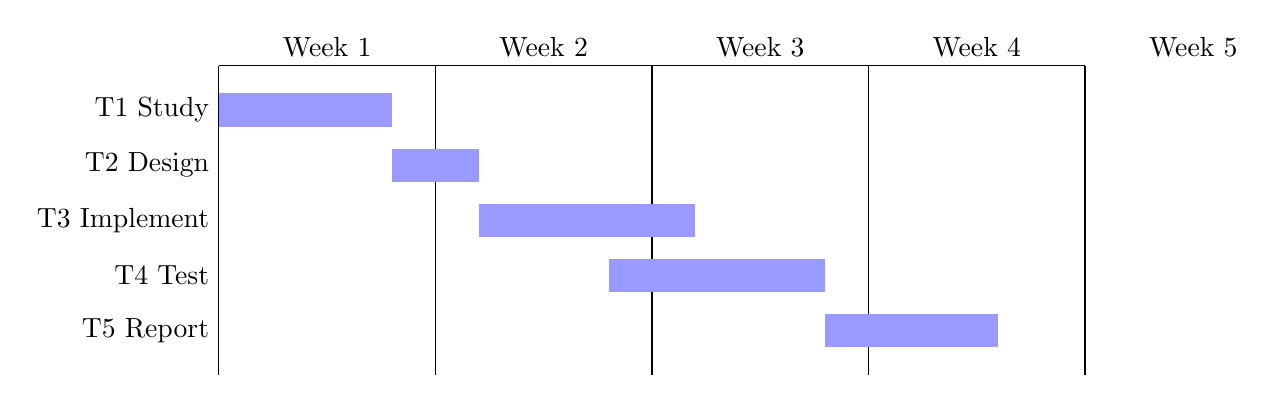
\begin{tikzpicture}[x=0.55cm,y=0.7cm]
  \foreach \w in {0,1,2,3,4} { \draw (\w*5,0.3) -- (\w*5,-5.3); \node[above] at (\w*5+2.5,0.3) {Week \the\numexpr\w+1\relax}; }
  \draw (0,0.3) -- (20,0.3);
  \node[left] at (0,-0.5) {T1 Study};      \fill[blue!40] (0,-0.8) rectangle (4,-0.2);
  \node[left] at (0,-1.5) {T2 Design};     \fill[blue!40] (4,-1.8) rectangle (6,-1.2);
  \node[left] at (0,-2.5) {T3 Implement};  \fill[blue!40] (6,-2.8) rectangle (11,-2.2);
  \node[left] at (0,-3.5) {T4 Test};       \fill[blue!40] (9,-3.8) rectangle (14,-3.2);
  \node[left] at (0,-4.5) {T5 Report};     \fill[blue!40] (14,-4.8) rectangle (18,-4.2);
\end{tikzpicture}
\caption{Project timeline (Gantt chart)}
\label{fig:gantt}
\end{figure}
Please refer to Annexure C for the planner.

\section{Team Organization}
\subsection{Team structure}
A flat team of four students with a shared repository. Roles: (1) parsing and timestamp logic, (2) acquisition, hashing and CLI, (3) reporting (CSV/HTML) and sample generator, (4) testing and documentation. All members reviewed each other's code through GitHub commits.

\subsection{Management reporting and communication}
Weekly progress was shown to the guide during the LP-IV laboratory slot. Day-to-day communication used a group chat, and all work was tracked through commits in the GitHub repository.

% =====================================================================
\chapter{Software requirement specification}

\section{Introduction}
\subsection{Purpose and Scope of Document}
This SRS describes the functional and non-functional requirements of the Browser History Forensic Analysis Tool so that it can be implemented, tested and evaluated. It covers acquisition, parsing, analysis and reporting of Chromium browser history.

\subsection{Overview of responsibilities of Developer}
The developers study the History schema, implement the tool, write a sample-database generator and automated tests, verify the tool on real data, and document the result.

\section{Usage Scenario}
\subsection{User profiles}
\begin{itemize}
  \item \textbf{Forensic examiner / investigator:} runs the tool on a seized History file or on a live profile and reads the report.
  \item \textbf{Student / learner:} runs the tool on the sample database to understand browser artifacts.
\end{itemize}

\subsection{Use-cases}
\begin{table}[H]
\begin{center}
\def\arraystretch{1.5}
\begin{tabularx}{\textwidth}{| c | l | X | c | X |}
\hline
Sr No.	& Use Case	& Description	& Actors	& Assumptions \\
\hline
1& Acquire evidence & Copy History file and compute SHA-256 & Examiner & Examiner has read access to the profile folder \\
\hline
2& Build timeline & Parse visits and show them in time order & Examiner & File is a valid Chromium History DB \\
\hline
3& Search keyword & List visits whose URL/title contains a word & Examiner & Keyword given on the command line \\
\hline
4& View statistics & Top domains and daily activity counts & Examiner & At least one visit exists \\
\hline
5& List downloads & Show downloaded files with source URL & Examiner & \texttt{downloads} table present \\
\hline
6& Export report & Write CSV and HTML report & Examiner & Output folder is writable \\
\hline
\end{tabularx}
\end{center}
\caption{Use Cases}
\label{tab:usecase}
\end{table}

\subsection{Use Case View}
\begin{figure}[H]
\centering
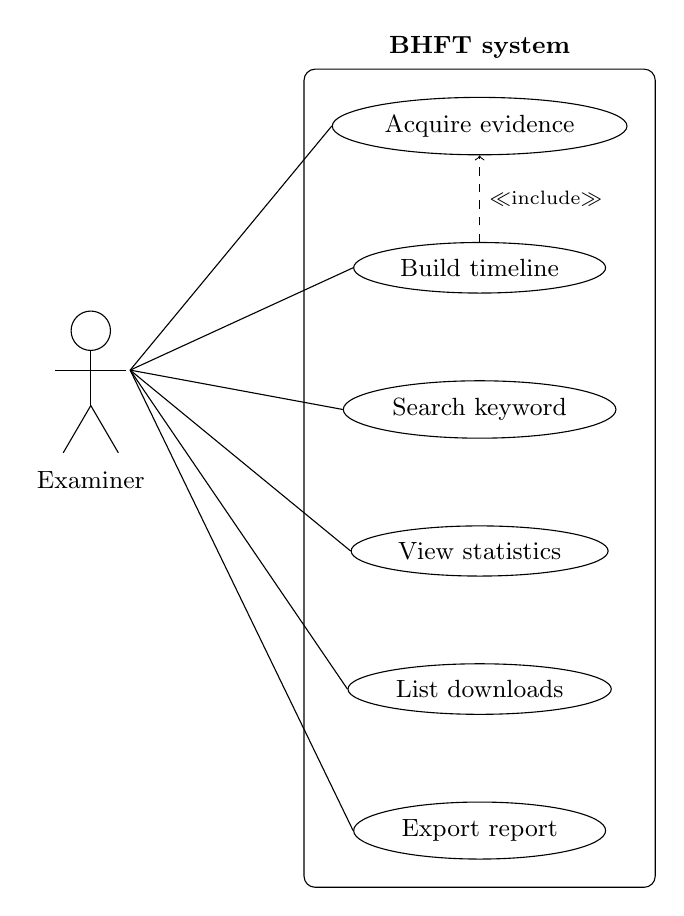
\begin{tikzpicture}[node distance=1.1cm, every node/.style={font=\small}]
  \node[draw, ellipse, minimum width=3.2cm] (u1) {Acquire evidence};
  \node[draw, ellipse, minimum width=3.2cm, below=of u1] (u2) {Build timeline};
  \node[draw, ellipse, minimum width=3.2cm, below=of u2] (u3) {Search keyword};
  \node[draw, ellipse, minimum width=3.2cm, below=of u3] (u4) {View statistics};
  \node[draw, ellipse, minimum width=3.2cm, below=of u4] (u5) {List downloads};
  \node[draw, ellipse, minimum width=3.2cm, below=of u5] (u6) {Export report};
  \node[draw, rounded corners, fit=(u1)(u6), inner sep=10pt, label=above:{\textbf{BHFT system}}] (sys) {};
  \coordinate (ah) at ($(u3.west)+(-3.2cm,1.0cm)$);
  \draw (ah) circle (0.25);
  \draw ($(ah)+(0,-0.25)$) -- ++(0,-0.7);
  \draw ($(ah)+(-0.45,-0.5)$) -- ++(0.9,0);
  \draw ($(ah)+(0,-0.95)$) -- ++(-0.35,-0.6);
  \draw ($(ah)+(0,-0.95)$) -- ++(0.35,-0.6);
  \node at ($(ah)+(0,-1.9)$) {Examiner};
  \coordinate (act) at ($(ah)+(0.5,-0.5)$);
  \foreach \u in {u1,u2,u3,u4,u5,u6} \draw (act) -- (\u.west);
  \draw[dashed,->] (u2) -- (u1) node[midway,right] {\scriptsize $\ll$include$\gg$};
\end{tikzpicture}
\caption{Use case diagram}
\label{fig:usecase}
\end{figure}

\section{Data Model and Description}
\subsection{Data Description}
The tool reads three tables of the Chromium History database (Table \ref{tab:schema}) and produces a list of \emph{visit records} and \emph{download records} in memory, which are then written to CSV and HTML.

\begin{table}[!htbp]
\begin{center}
\def\arraystretch{1.4}
\begin{tabularx}{\textwidth}{| l | l | X |}
\hline
Table & Column & Meaning \\ \hline
\texttt{urls} & id, url, title, visit\_count, typed\_count, last\_visit\_time & one row per unique URL \\ \hline
\texttt{visits} & id, url (FK to urls.id), visit\_time, from\_visit, transition & one row per visit \\ \hline
\texttt{downloads} & id, target\_path, tab\_url, start\_time, received\_bytes & one row per download \\ \hline
\end{tabularx}
\end{center}
\caption{Chromium History tables used by the tool}
\label{tab:schema}
\end{table}

\subsection{Data objects and Relationships}
\begin{figure}[H]
\centering
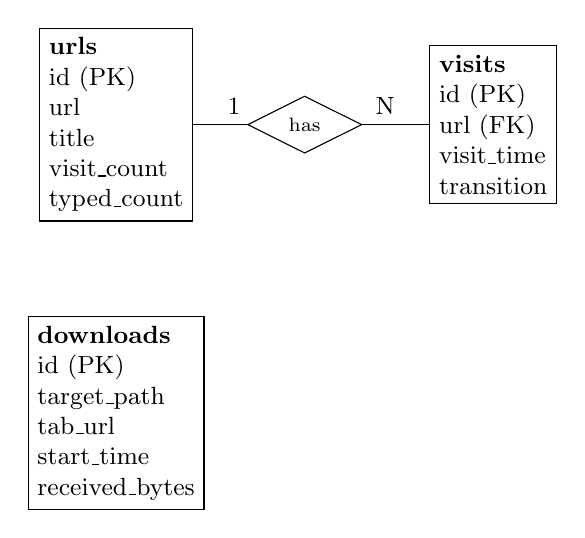
\begin{tikzpicture}[node distance=2.2cm, every node/.style={font=\small}]
  \node[draw, rectangle, align=left] (urls) {\textbf{urls}\\ id (PK)\\ url\\ title\\ visit\_count\\ typed\_count};
  \node[draw, rectangle, align=left, right=3cm of urls] (visits) {\textbf{visits}\\ id (PK)\\ url (FK)\\ visit\_time\\ transition};
  \node[draw, rectangle, align=left, below=1.2cm of urls] (dl) {\textbf{downloads}\\ id (PK)\\ target\_path\\ tab\_url\\ start\_time\\ received\_bytes};
  \draw (urls) -- node[above] {1 \hspace{1.5cm} N} (visits);
  \node[draw, diamond, aspect=2, fill=white, font=\scriptsize] at ($(urls)!0.5!(visits)$) {has};
\end{tikzpicture}
\caption{Entity relationship of the History tables}
\label{fig:erd}
\end{figure}

\section{Functional Model and Description}
\subsection{Data Flow Diagram}
\subsubsection{Level 0 Data Flow Diagram}
\begin{figure}[H]
\centering
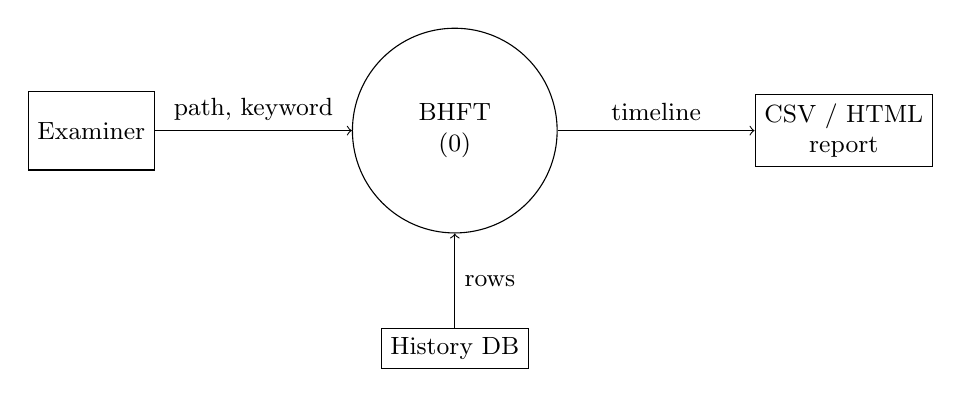
\begin{tikzpicture}[node distance=2.5cm, every node/.style={font=\small}]
  \node[draw, rectangle, minimum height=1cm] (ex) {Examiner};
  \node[draw, circle, minimum size=2.6cm, align=center, right=of ex] (p) {BHFT\\(0)};
  \node[draw, rectangle, align=center, right=of p] (rep) {CSV / HTML\\report};
  \node[draw, rectangle, below=1.2cm of p] (db) {History DB};
  \draw[->] (ex) -- node[above] {path, keyword} (p);
  \draw[->] (db) -- node[right] {rows} (p);
  \draw[->] (p) -- node[above] {timeline} (rep);
\end{tikzpicture}
\caption{Level 0 DFD}
\label{fig:dfd0}
\end{figure}

\subsubsection{Level 1 Data Flow Diagram}
\begin{figure}[H]
\centering
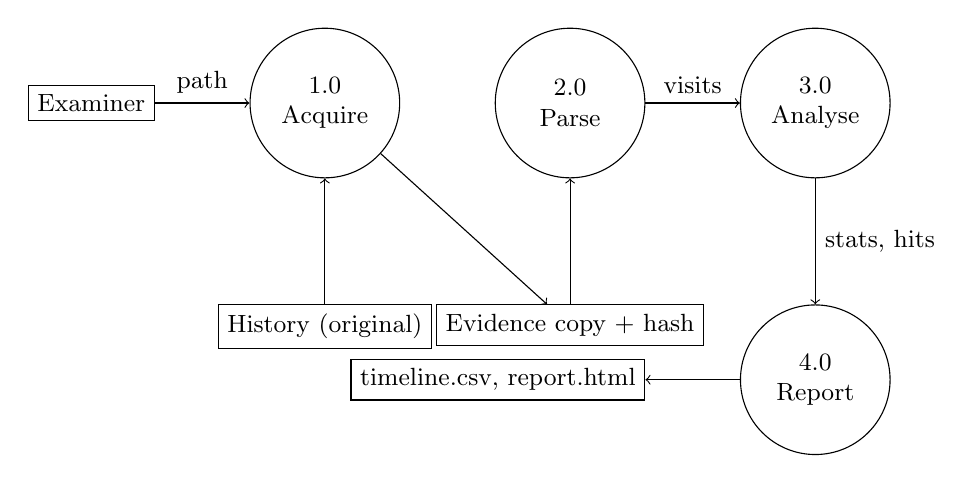
\begin{tikzpicture}[node distance=1.6cm and 1.2cm, every node/.style={font=\small}]
  \node[draw, rectangle] (ex) {Examiner};
  \node[draw, circle, minimum size=1.9cm, align=center, right=of ex] (p1) {1.0\\Acquire};
  \node[draw, circle, minimum size=1.9cm, align=center, right=of p1] (p2) {2.0\\Parse};
  \node[draw, circle, minimum size=1.9cm, align=center, right=of p2] (p3) {3.0\\Analyse};
  \node[draw, circle, minimum size=1.9cm, align=center, below=of p3] (p4) {4.0\\Report};
  \node[draw, rectangle, below=of p1] (src) {History (original)};
  \node[draw, rectangle, below=of p2] (copy) {Evidence copy + hash};
  \node[draw, rectangle, left=of p4] (out) {timeline.csv, report.html};
  \draw[->] (ex) -- node[above] {path} (p1);
  \draw[->] (src) -- (p1);
  \draw[->] (p1) -- (copy);
  \draw[->] (copy) -- (p2);
  \draw[->] (p2) -- node[above] {visits} (p3);
  \draw[->] (p3) -- node[right] {stats, hits} (p4);
  \draw[->] (p4) -- (out);
\end{tikzpicture}
\caption{Level 1 DFD}
\label{fig:dfd1}
\end{figure}

\subsection{Activity Diagram:}
\begin{figure}[H]
\centering
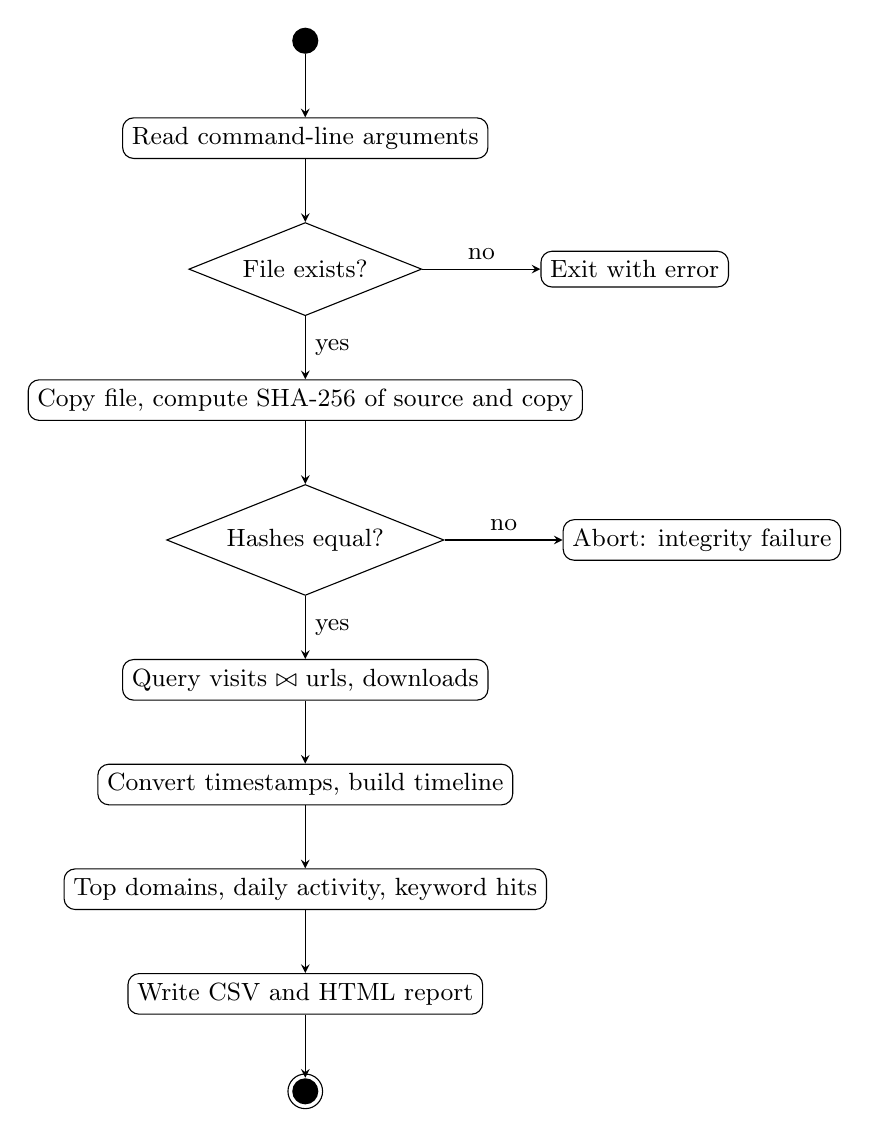
\begin{tikzpicture}[node distance=0.8cm, every node/.style={font=\small}, >=stealth]
  \node[circle, fill=black, minimum size=0.3cm] (s) {};
  \node[draw, rounded corners, below=of s] (a1) {Read command-line arguments};
  \node[draw, diamond, aspect=2.5, below=of a1] (d1) {File exists?};
  \node[draw, rounded corners, below=of d1] (a2) {Copy file, compute SHA-256 of source and copy};
  \node[draw, diamond, aspect=2.5, below=of a2] (d2) {Hashes equal?};
  \node[draw, rounded corners, below=of d2] (a3) {Query visits $\bowtie$ urls, downloads};
  \node[draw, rounded corners, below=of a3] (a4) {Convert timestamps, build timeline};
  \node[draw, rounded corners, below=of a4] (a5) {Top domains, daily activity, keyword hits};
  \node[draw, rounded corners, below=of a5] (a6) {Write CSV and HTML report};
  \node[circle, fill=black, minimum size=0.3cm, below=of a6] (e) {};
  \draw (e) circle (0.22cm);
  \node[draw, rounded corners, right=1.5cm of d1] (err1) {Exit with error};
  \node[draw, rounded corners, right=1.5cm of d2] (err2) {Abort: integrity failure};
  \draw[->] (s) -- (a1); \draw[->] (a1) -- (d1);
  \draw[->] (d1) -- node[right] {yes} (a2); \draw[->] (d1) -- node[above] {no} (err1);
  \draw[->] (a2) -- (d2);
  \draw[->] (d2) -- node[right] {yes} (a3); \draw[->] (d2) -- node[above] {no} (err2);
  \draw[->] (a3) -- (a4); \draw[->] (a4) -- (a5); \draw[->] (a5) -- (a6); \draw[->] (a6) -- (e);
\end{tikzpicture}
\caption{Activity diagram}
\label{fig:activity}
\end{figure}

\subsection{Non Functional Requirements:}
\begin{itemize}
  \item \textbf{Interface Requirements:} command-line interface with \texttt{--browser}, \texttt{--db}, \texttt{--out}, \texttt{--keyword}, \texttt{--top}; HTML report viewable in any browser.
  \item \textbf{Performance Requirements:} process a 100\,000-visit database in under 2 seconds on the minimum hardware.
  \item \textbf{Availability / Reliability:} no network dependency; deterministic output for the same input.
  \item \textbf{Modifiability / Portability:} single file, standard library only, runs on Windows, Linux and macOS.
  \item \textbf{Security:} the source file is opened read-only; the evidence copy is hash-verified.
  \item \textbf{Testability:} every function is unit-tested with pytest; an end-to-end test runs the CLI.
  \item \textbf{Usability:} one command produces all outputs; the report is self-explanatory.
\end{itemize}

\subsection{State Diagram:}
Fig.\ref{fig:state-dig} shows the states of the tool during one run.
\begin{figure}[H]
\centering
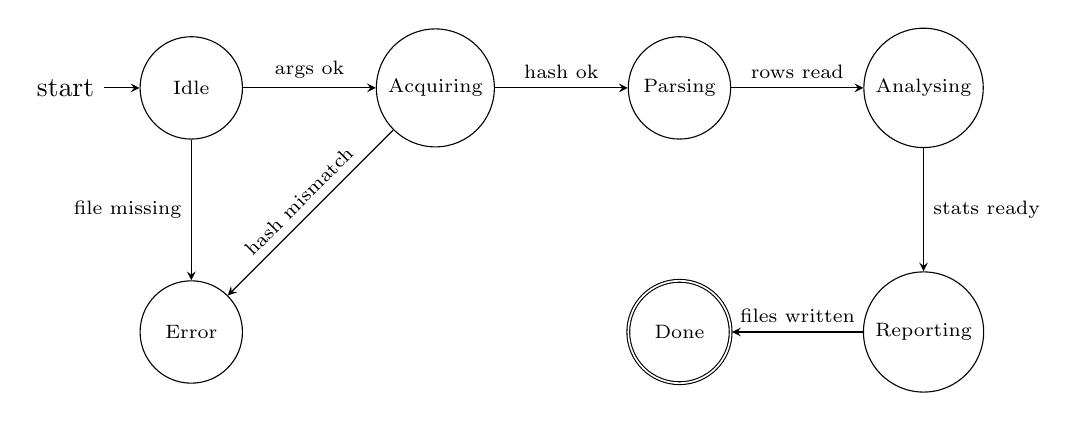
\begin{tikzpicture}[->, >=stealth, node distance=3.1cm, every state/.style={font=\scriptsize, minimum size=1.3cm}]
  \node[state, initial] (idle) {Idle};
  \node[state, right of=idle] (acq) {Acquiring};
  \node[state, right of=acq] (par) {Parsing};
  \node[state, right of=par] (ana) {Analysing};
  \node[state, below of=ana] (rep) {Reporting};
  \node[state, accepting, below of=par] (done) {Done};
  \node[state, below of=idle] (err) {Error};
  \path (idle) edge node[above, font=\scriptsize] {args ok} (acq)
        (acq) edge node[above, font=\scriptsize] {hash ok} (par)
        (par) edge node[above, font=\scriptsize] {rows read} (ana)
        (ana) edge node[right, font=\scriptsize] {stats ready} (rep)
        (rep) edge node[above, font=\scriptsize] {files written} (done)
        (acq) edge node[above, sloped, font=\scriptsize] {hash mismatch} (err)
        (idle) edge node[left, font=\scriptsize] {file missing} (err);
\end{tikzpicture}
\caption{State transition diagram}
\label{fig:state-dig}
\end{figure}

\subsection{Design Constraints}
Standard library only; no modification of the source file; output must be plain CSV and HTML so that it can be opened on any machine.

\subsection{Software Interface Description}
\begin{itemize}
  \item \textbf{Input interface:} file system (History file) and command-line arguments.
  \item \textbf{Database interface:} Python \texttt{sqlite3} module, opened with the URI \texttt{file:...?mode=ro}.
  \item \textbf{Output interface:} files in the output folder; console summary on standard output.
\end{itemize}

% =====================================================================
\chapter{Detailed Design Document using Appendix A and B}
\section{Introduction}
This chapter describes the architecture, data design and component design used to implement the tool.

\section{Architectural Design}
The tool is a linear pipeline of four modules inside one Python file (Fig.\ref{fig:arch-dig}), mirroring the NIST forensic process.
\begin{figure}[H]
\centering
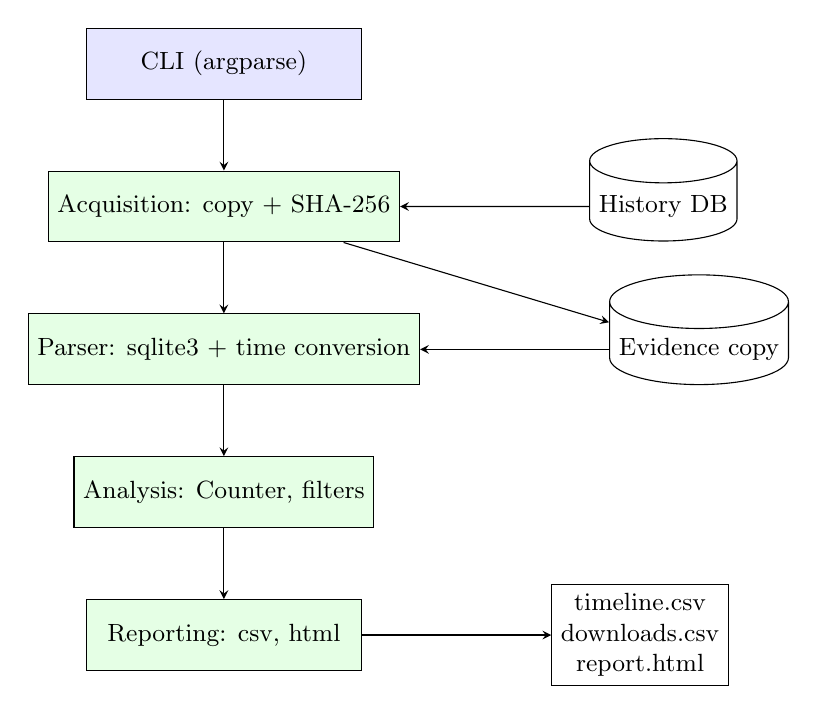
\begin{tikzpicture}[node distance=0.9cm, every node/.style={font=\small}, >=stealth]
  \node[draw, fill=blue!10, minimum width=3.5cm, minimum height=0.9cm] (cli) {CLI (argparse)};
  \node[draw, fill=green!10, minimum width=3.5cm, minimum height=0.9cm, below=of cli] (acq) {Acquisition: copy + SHA-256};
  \node[draw, fill=green!10, minimum width=3.5cm, minimum height=0.9cm, below=of acq] (par) {Parser: sqlite3 + time conversion};
  \node[draw, fill=green!10, minimum width=3.5cm, minimum height=0.9cm, below=of par] (ana) {Analysis: Counter, filters};
  \node[draw, fill=green!10, minimum width=3.5cm, minimum height=0.9cm, below=of ana] (rep) {Reporting: csv, html};
  \node[draw, cylinder, shape border rotate=90, aspect=0.3, minimum height=1.3cm, right=2.4cm of acq] (hist) {History DB};
  \node[draw, cylinder, shape border rotate=90, aspect=0.3, minimum height=1.3cm, right=2.4cm of par] (copy) {Evidence copy};
  \node[draw, right=2.4cm of rep, align=center] (out) {timeline.csv\\downloads.csv\\report.html};
  \draw[->] (cli) -- (acq); \draw[->] (acq) -- (par); \draw[->] (par) -- (ana); \draw[->] (ana) -- (rep);
  \draw[->] (hist) -- (acq); \draw[->] (acq) -- (copy); \draw[->] (copy) -- (par); \draw[->] (rep) -- (out);
\end{tikzpicture}
\caption{Architecture diagram}
\label{fig:arch-dig}
\end{figure}

\section{Data design (using Appendices A and B)}
\subsection{Internal software data structure}
A \emph{visit record} is a Python dictionary with keys \texttt{time}, \texttt{url}, \texttt{title}, \texttt{domain}, \texttt{visit\_count}, \texttt{typed\_count}. A \emph{download record} has \texttt{time}, \texttt{file}, \texttt{url}, \texttt{bytes}. Both are passed between the parse, analyse and report functions as lists.
\subsection{Global data structure}
\texttt{WEBKIT\_EPOCH\_DELTA = 11644473600}, the constant used for timestamp conversion, and the dictionary of default profile paths per browser and operating system.
\subsection{Temporary data structure}
\texttt{collections.Counter} objects for domain and daily frequencies; the list of HTML fragments assembled before writing the report.
\subsection{Database description}
The input is the Chromium History SQLite database (Table \ref{tab:schema}). The tool creates no database of its own; the evidence copy \texttt{History\_evidence\_copy.db} is a byte-for-byte copy of the input.

\section{Component Design}
\subsection{Class Diagram}
The implementation is procedural, but its functions group naturally into four components shown as classes in Fig.\ref{fig:class-dig}.
\begin{figure}[H]
\centering
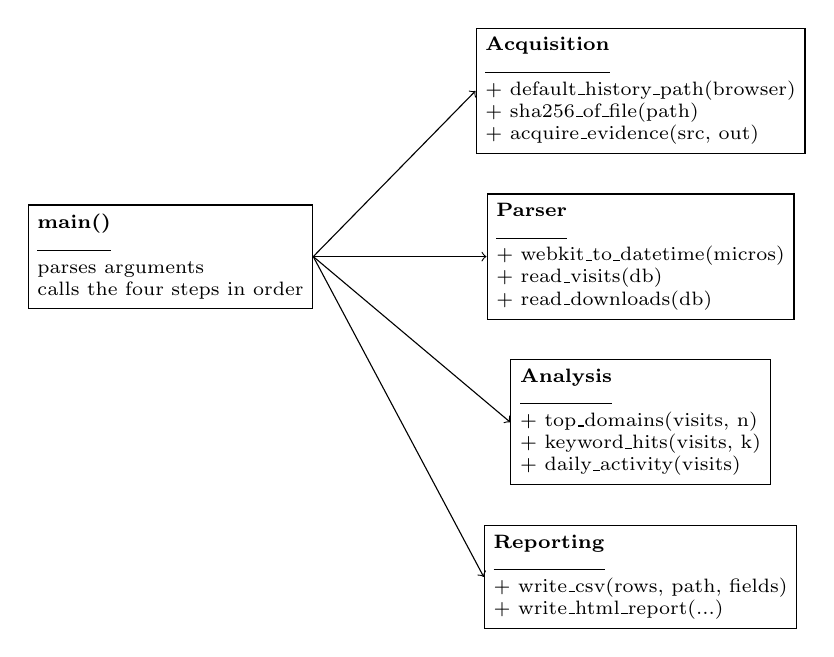
\begin{tikzpicture}[node distance=0.5cm and 2.2cm, every node/.style={font=\scriptsize}]
  \node[draw, rectangle, align=left] (acq) {\textbf{Acquisition}\\ \hrulefill\\ + default\_history\_path(browser)\\ + sha256\_of\_file(path)\\ + acquire\_evidence(src, out)};
  \node[draw, rectangle, align=left, below=of acq] (par) {\textbf{Parser}\\ \hrulefill\\ + webkit\_to\_datetime(micros)\\ + read\_visits(db)\\ + read\_downloads(db)};
  \node[draw, rectangle, align=left, below=of par] (ana) {\textbf{Analysis}\\ \hrulefill\\ + top\_domains(visits, n)\\ + keyword\_hits(visits, k)\\ + daily\_activity(visits)};
  \node[draw, rectangle, align=left, below=of ana] (rep) {\textbf{Reporting}\\ \hrulefill\\ + write\_csv(rows, path, fields)\\ + write\_html\_report(...)};
  \node[draw, rectangle, align=left, left=of par] (main) {\textbf{main()}\\ \hrulefill\\ parses arguments\\ calls the four steps in order};
  \draw[->] (main.east) -- (acq.west); \draw[->] (main.east) -- (par.west); \draw[->] (main.east) -- (ana.west); \draw[->] (main.east) -- (rep.west);
\end{tikzpicture}
\caption{Class / component diagram}
\label{fig:class-dig}
\end{figure}

% =====================================================================
\chapter{Project Implementation}
\section{Introduction}
The tool was implemented as a single script \texttt{bhft.py} (about 280 lines), with a helper script \texttt{make\_sample\_db.py} that generates a realistic synthetic History database and a test module \texttt{test\_bhft.py}. The code is hosted at \url{https://github.com/VishwajeetTulse/browser-history-forensic-tool}.

\section{Tools and Technologies Used}
\begin{itemize}
  \item Python 3.14 (standard library: \texttt{sqlite3}, \texttt{hashlib}, \texttt{csv}, \texttt{argparse}, \texttt{datetime}, \texttt{shutil}, \texttt{html}, \texttt{collections})
  \item pytest 9 for automated tests
  \item Git and GitHub for version control
  \item Visual Studio Code; Microsoft Edge (live test profile and report viewing)
\end{itemize}

\section{Methodologies/Algorithm Details}
\subsection{Algorithm 1/Pseudo Code}
\begin{algorithm}[H]
\caption{Evidence acquisition with integrity check}
\KwIn{source path $src$, output folder $out$}
\KwOut{copy path $dst$, digest $h$}
create $out$ if missing\;
$dst \leftarrow out/\texttt{History\_evidence\_copy.db}$\;
byte-copy $src$ to $dst$\;
$h_s \leftarrow \mathrm{SHA256}(src)$; $h_d \leftarrow \mathrm{SHA256}(dst)$\;
\If{$h_s \neq h_d$}{abort with ``integrity cannot be guaranteed''\;}
\Return $(dst, h_s)$\;
\end{algorithm}

\subsection{Algorithm 2/Pseudo Code}
\begin{algorithm}[H]
\caption{Timeline construction and analysis}
\KwIn{evidence copy $dst$, keyword $k$, count $n$}
\KwOut{timeline $T$, top domains $D$, hits $K$, daily counts $A$}
open $dst$ read-only\;
rows $\leftarrow$ \texttt{SELECT v.visit\_time, u.url, u.title, u.visit\_count, u.typed\_count FROM visits v JOIN urls u ON v.url=u.id ORDER BY v.visit\_time}\;
\ForEach{row in rows}{
  $t \leftarrow$ row.visit\_time$/10^6 - 11644473600$ seconds since 1970, converted to local time\;
  append (t, url, title, domain(url), counts) to $T$\;
}
$D \leftarrow$ $n$ most common domains in $T$\;
$K \leftarrow \{v \in T : k \in \mathrm{lower}(v.url) \lor k \in \mathrm{lower}(v.title)\}$\;
$A \leftarrow$ count of visits per calendar date\;
\Return $(T, D, K, A)$\;
\end{algorithm}

Key implementation of the timestamp conversion:
\begin{lstlisting}[language=Python]
WEBKIT_EPOCH_DELTA = 11644473600  # seconds between 1601-01-01 and 1970-01-01

def webkit_to_datetime(micros):
    """Chromium stores times as microseconds since 1601-01-01 UTC."""
    if not micros:
        return None
    seconds = micros / 1_000_000 - WEBKIT_EPOCH_DELTA
    return dt.datetime.fromtimestamp(seconds, dt.timezone.utc).astimezone()
\end{lstlisting}

\section{Verification and Validation for Acceptance}
Acceptance criteria: (a) hash of copy equals hash of source, (b) timeline is in increasing time order, (c) all visits in the database appear in the timeline, (d) keyword search is case-insensitive, (e) CSV and HTML files are produced. All criteria are checked automatically by the pytest suite (Chapter 9) and were also confirmed manually on a live Microsoft Edge profile.

% =====================================================================
\chapter{Software Testing}
\section{Type of Testing Used}
\begin{itemize}
  \item \textbf{Unit testing} of individual functions (timestamp conversion, hashing, parsing, analysis) with pytest.
  \item \textbf{Integration / end-to-end testing} by running the complete CLI on the sample database and checking the output files.
  \item \textbf{System testing} by running the tool against the live Microsoft Edge profile of a Windows 11 machine.
\end{itemize}

\section{Test Cases and Test Results}
\begin{table}[!htbp]
\begin{center}
\def\arraystretch{1.4}
\begin{tabularx}{\textwidth}{| c | X | X | c |}
\hline
TC & Test description & Expected result & Result \\ \hline
TC1 & Convert WebKit value of Unix epoch & 1970-01-01; value 0 gives None & Pass \\ \hline
TC2 & SHA-256 of sample file & equals hashlib digest & Pass \\ \hline
TC3 & Read visits from sample DB & non-empty, sorted by time, every row has a domain & Pass \\ \hline
TC4 & Read downloads & 3 rows, first is a .pdf & Pass \\ \hline
TC5 & Keyword search ``BANK'' vs ``bank'' & same hits; unknown keyword gives empty list & Pass \\ \hline
TC6 & Top-3 domains & 3 entries in non-increasing order & Pass \\ \hline
TC7 & End-to-end CLI run with \texttt{--keyword bank} & exit 0; report.html, timeline.csv, evidence copy exist; ``SHA-256'' printed & Pass \\ \hline
TC8 & System test on live Edge profile & tool copies locked file, prints hash and timeline & Pass \\ \hline
\end{tabularx}
\end{center}
\caption{Test cases and results}
\label{tab:tests}
\end{table}

pytest output:
\begin{lstlisting}
test_bhft.py::test_webkit_epoch_conversion PASSED
test_bhft.py::test_sha256_matches_hashlib PASSED
test_bhft.py::test_read_visits_sorted_and_complete PASSED
test_bhft.py::test_downloads_read PASSED
test_bhft.py::test_keyword_search_case_insensitive PASSED
test_bhft.py::test_top_domains_order PASSED
test_bhft.py::test_end_to_end_cli PASSED
============================== 7 passed in 0.21s ==============================
\end{lstlisting}

% =====================================================================
\chapter{Results}
\section{Screen shots}
\begin{figure}[H]
\centering
\fbox{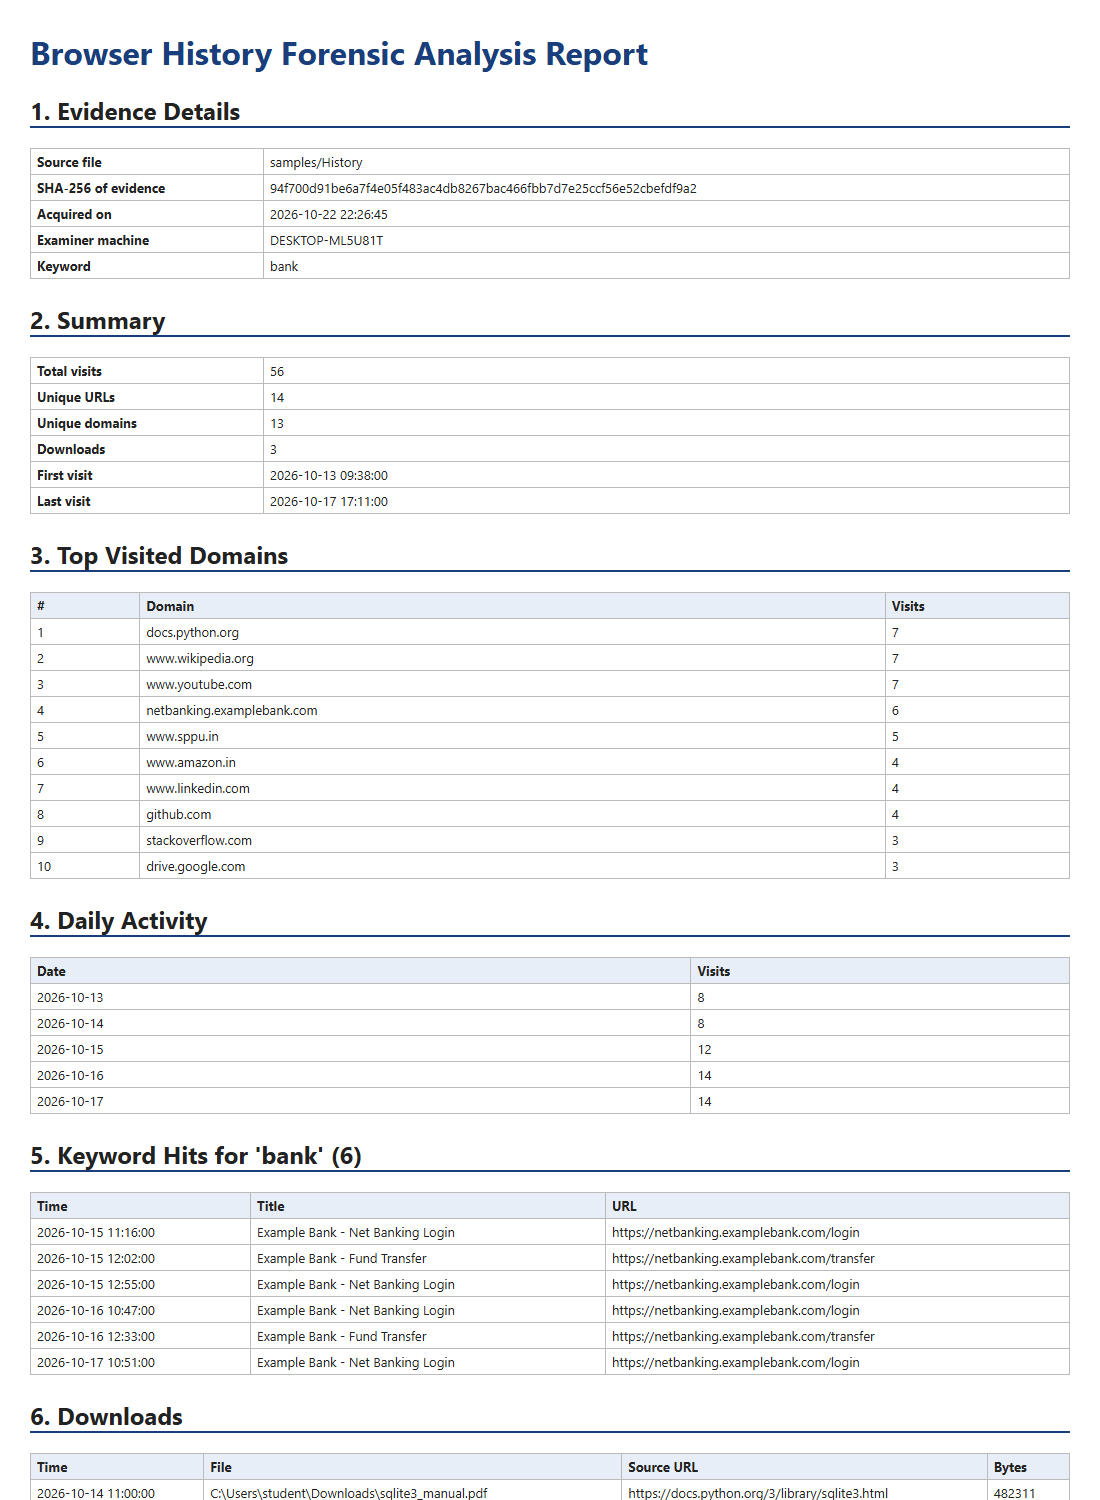
\includegraphics[width=0.95\textwidth]{figures/report_html.png}}
\caption{Generated HTML forensic report (sample database, keyword ``bank'')}
\label{fig:report}
\end{figure}

\section{Outputs}
Console output of \texttt{python bhft.py --db samples/History --out output --keyword bank}:
\begin{lstlisting}
======================================================================
 Browser History Forensic Analysis Tool
======================================================================
[1] Acquiring evidence from: samples/History
    SHA-256 : 94f700d91be6a7f4e05f483ac4db8267bac466fbb7d7e25ccf56e52cbefdf9a2
    Working copy saved to: output\History_evidence_copy.db
[2] Parsing history database ...
    56 visits, 3 downloads found
[3] Analysing ...

    Top 10 domains:
          7  docs.python.org
          7  www.wikipedia.org
          7  www.youtube.com
          6  netbanking.examplebank.com
          5  www.sppu.in
          4  www.amazon.in
          4  www.linkedin.com
          4  github.com
          3  stackoverflow.com
          3  drive.google.com

    Activity window: 2026-10-13 09:38:00  ->  2026-10-17 17:11:00

    Keyword 'bank': 6 hit(s)
      2026-10-15 11:16:00  https://netbanking.examplebank.com/login
      2026-10-15 12:02:00  https://netbanking.examplebank.com/transfer
      2026-10-15 12:55:00  https://netbanking.examplebank.com/login
      2026-10-16 10:47:00  https://netbanking.examplebank.com/login
      2026-10-16 12:33:00  https://netbanking.examplebank.com/transfer
      2026-10-17 10:51:00  https://netbanking.examplebank.com/login

[4] Writing reports ...
    timeline.csv, downloads.csv and report.html written to 'output'
Done.
\end{lstlisting}

First rows of \texttt{timeline.csv}:
\begin{lstlisting}
time,url,title,domain,visit_count,typed_count
2026-10-13 09:38:00,https://www.amazon.in/,Amazon.in,www.amazon.in,4,2
2026-10-13 09:44:00,https://www.linkedin.com/feed/,Feed | LinkedIn,www.linkedin.com,4,0
\end{lstlisting}

% =====================================================================
\chapter{Deployment and Maintenance}
\section{Installation and un-installation}
\begin{enumerate}
  \item Install Python 3.9 or newer.
  \item Clone the repository from \url{https://github.com/VishwajeetTulse/browser-history-forensic-tool}
  \item (Optional) \texttt{pip install pytest} to run the tests.
  \item Un-installation: delete the folder. The tool writes nothing outside its output directory.
\end{enumerate}
\section{User help}
\begin{lstlisting}
python make_sample_db.py                       # create demo database
python bhft.py --db samples/History --keyword bank
python bhft.py --browser edge                  # live Edge profile
python bhft.py --browser chrome --out case42 --top 20
python bhft.py --help                          # all options
\end{lstlisting}
Open \texttt{output/report.html} in a browser. Keep \texttt{History\_evidence\_copy.db} together with the printed SHA-256 value as part of the case record.

% =====================================================================
\chapter{Conclusion and Future Scope}
The Browser History Forensic Analysis Tool demonstrates, in a small and transparent way, the complete forensic workflow for a common digital artifact. It acquires the Chromium History database without touching the original, proves integrity with SHA-256, decodes WebKit timestamps, reconstructs a chronological timeline and summarises the activity in a report that an investigator can use directly. All functions are covered by automated tests and the tool was validated on real browser data.

Future scope includes support for Firefox (\texttt{places.sqlite}) and Safari, parsing of cookies, cache and form data, recovery of deleted records from SQLite free pages, a graphical interface, and correlation of several users' timelines in one case.

% =====================================================================
\begin{thebibliography}{99}
\bibitem{oh2011} J. Oh, S. Lee and S. Lee. 2011. Advanced evidence collection and analysis of web browser activity. \emph{Digital Investigation} 8 (2011), S62--S70.
\bibitem{ohana2013} D. J. Ohana and N. Shashidhar. 2013. Do private and portable web browsers leave incriminating evidence? A forensic analysis of residual artifacts from private and portable web browsing sessions. \emph{EURASIP Journal on Information Security} 2013, 6.
\bibitem{rathod2017} D. Rathod. 2017. Web browser forensics: Google Chrome. \emph{International Journal of Advanced Research in Computer Science} 8, 7 (2017), 896--899.
\bibitem{casey2011} E. Casey. 2011. \emph{Digital Evidence and Computer Crime} (3rd ed.). Academic Press.
\bibitem{carrier2005} B. Carrier. 2005. \emph{File System Forensic Analysis}. Addison-Wesley.
\bibitem{nist80086} K. Kent, S. Chevalier, T. Grance and H. Dang. 2006. \emph{Guide to Integrating Forensic Techniques into Incident Response}. NIST Special Publication 800-86.
\bibitem{kessler2016} G. C. Kessler. 2016. An overview of cryptographic hash functions and their uses in digital forensics. \emph{Journal of Digital Forensics, Security and Law}.
\bibitem{chromiumhist} The Chromium Projects. \emph{User Data Directory and History database design}. \url{https://www.chromium.org/developers/design-documents/user-data-dir/}
\bibitem{sqlite} SQLite Consortium. \emph{SQLite Documentation: Database File Format and URI Filenames}. \url{https://www.sqlite.org/docs.html}
\bibitem{pydocs} Python Software Foundation. \emph{The Python Standard Library: sqlite3, hashlib, datetime}. \url{https://docs.python.org/3/library/}
\bibitem{bookPressman} R. S. Pressman. 2010. \emph{Software Engineering: A Practitioner's Approach} (7th ed.). McGraw-Hill.
\end{thebibliography}

% =====================================================================
\begin{appendices}

\chapter{Laboratory assignments on Project Analysis of Algorithmic Design}
\begin{itemize}
\item \textbf{IDEA Matrix.} Increase: investigator productivity. Drive: evidence-based conclusions. Educate: students on artifact structure. Accelerate: timeline reconstruction. Improve: integrity assurance via hashing. Deliver: CSV/HTML reports. Evaluate: browsing patterns (top domains, daily activity). Associate: downloads with their source pages. Ignore: cosmetics (GUI). Decrease: manual SQL work. Eliminate: risk of altering original evidence. Avoid: third-party dependencies.
\item \textbf{Feasibility.} All operations are polynomial: SQL join with sort $O(m \log m)$, analysis passes $O(m)$, hashing $O(\text{file size})$. The problem is in P; there is no NP-hard component.
\item \textbf{Function.} $x$ = History file, $y = f(x) = (h, T, D, K, L)$ where $h$ is the hash, $T$ the timeline, $D$ the domain table, $K$ the keyword hits and $L$ the download list.
\end{itemize}

\chapter{Laboratory assignments on Project Quality and Reliability Testing of Project Design}
\begin{itemize}
\item \textbf{Objects and morphisms.} Objects: History file, visit record, download record, report. Morphisms: acquire (file $\to$ copy + hash), parse (copy $\to$ records), analyse (records $\to$ statistics), report (statistics $\to$ files). The functions are composed sequentially: $\mathrm{report} \circ \mathrm{analyse} \circ \mathrm{parse} \circ \mathrm{acquire}$.
\item \textbf{Functional dependency graph.} report depends on analyse; analyse depends on parse; parse depends on acquire. No cycles; see the DFD in Fig.\ref{fig:dfd1}.
\item \textbf{Black-box test data.} Generated by \texttt{make\_sample\_db.py} with a fixed random seed (56 visits over 5 days, 3 downloads, one domain containing the keyword ``bank'').
\item \textbf{Black-box test cases.} Listed in Table \ref{tab:tests}.
\end{itemize}

\chapter{Project Planner}
\label{app:plan}
\begin{table}[H]
\begin{center}
\def\arraystretch{1.3}
\begin{tabularx}{\textwidth}{| c | X | c | c |}
\hline
Week & Activity & Deliverable & Status \\ \hline
1 & Study Chromium History schema, WebKit timestamps, NIST 800-86 & Notes, design sketch & Done \\ \hline
2 & Implement acquisition, parser, CLI; sample DB generator & \texttt{bhft.py} v0.1 & Done \\ \hline
3 & Analysis and reporting; pytest suite; live Edge test & \texttt{bhft.py} v1.0, tests & Done \\ \hline
4 & README, GitHub repository, project report & Repository, report & Done \\ \hline
\end{tabularx}
\end{center}
\caption{Project planner}
\end{table}

\chapter{Reviewers Comments of Paper Submitted}
Not applicable for this mini project.

\chapter{Plagiarism Report}
To be attached after checking through the institute's plagiarism tool.

\chapter{Term-II Project Laboratory Assignments}
\begin{enumerate}
\item Review of design: the design was reviewed with the guide; the suggestion to add hash verification of the copy was incorporated.
\item Project workstation: Windows 11 laptop with Python 3.14, VS Code, Git and Microsoft Edge; setup took under 30 minutes.
\item Programming: completed as described in Chapter 8.
\item Testing: pytest suite of seven tests and a live-profile system test; results in Chapter 9.
\end{enumerate}

\chapter{Information of Project Group Members}
\begin{enumerate}
\item Name : Vishwajeet Tulse
\item Date of Birth :
\item Gender :
\item Permanent Address :
\item E-Mail :
\item Mobile/Contact No. :
\item Placement Details :
\item Paper Published : --
\end{enumerate}
\newpage
\begin{enumerate}
\item Name : Student Name 2
\item Date of Birth :
\item Gender :
\item Permanent Address :
\item E-Mail :
\item Mobile/Contact No. :
\item Placement Details :
\item Paper Published : --
\end{enumerate}
\newpage
\begin{enumerate}
\item Name : Student Name 3
\item Date of Birth :
\item Gender :
\item Permanent Address :
\item E-Mail :
\item Mobile/Contact No. :
\item Placement Details :
\item Paper Published : --
\end{enumerate}
\newpage
\begin{enumerate}
\item Name : Student Name 4
\item Date of Birth :
\item Gender :
\item Permanent Address :
\item E-Mail :
\item Mobile/Contact No. :
\item Placement Details :
\item Paper Published : --
\end{enumerate}
\end{appendices}

\end{document}
